\ifdefined\COMPLETE
\else
    \input{./preambule-sacha-utf8.ltx}
    \begin{document}
\fi


\section{Équations à une inconnue}

\subsection{Équations du premier degré}

\textbf{Exemple \no 0}

$ 2x - 3 = 0 $ \\

Résoudre l'équation $ 2x-3=0$

c'est trouver l'\textbf{ensemble} des nombres réels x tels que $2x-3=0$ \\

$ 2x-3=0$

$ 2x-3+3 = 0+3$ 

$2x=3$ \\

$ 2x \times \dfrac{1}{2} = 3 \times \dfrac{1}{2} $ \\

$ x = \dfrac{3}{2} $ \\

$ S = \left\lbrace\dfrac{3}{2}\right\rbrace $ \\

\textbf{Remarque}

Un ensemble ne contenant qu'un élément s'appelle un \textbf{singleton} \\

\textbf{Exemple \no 1}

$ 3x-5=9x+1 $

$ 3x-9x=1+5 $

$-6x=6 $

$6x=-6 $

$x = -1 $ \\

$ S = \left\lbrace-1\right\rbrace $ \\

\textbf{Exemple \no 2}

$ 6-4\left(1-x\right) = 4x+5 $

$ 6 - 4 + 4x = 4x + 5 $

$ 4x - 4x = 5 -6 + 4 $

$ 0x = 3  $ \\

L'équation n'admet aucune solution, donc : 

$ S = \varnothing $ \\

\textbf{Exemple \no 3}

$ 3 - \left[5-\left(2x-7\right)\right] = 2\left(x-4\right)-1 $

$ 3 - \left(5-2x+7\right) = 2x - 8 - 1 $ 

$ 3 - 5 + 2x - 7 = 2x - 8 -1 $

$ 2x - 2x = -8 -1 -3 + 5 + 7 $

$ 0x = 0 $ 

L'équation admet une infinité de solutions, donc :

$ S = \R $ 

\subsection{Équations produit}

\textbf{Exemple \no 0}

\vspace{.1cm}

$ \left(2x+5\right)\left(x-3\right)=0 $

Trouver l'ensemble des nombres réels x tels que $\left(2x+5\right)\left(x-3\right)=0 $ \\

\begin{tabular}{lcl}
$ 2x + 5 = 0 $ &  ou   & $ x-3 = 0 $ \\
&&\\
$ 2x = -5 $ & ou & $ x=3 $\\ 
&&\\
$x = -\dfrac{5}{2} $ &&\\
\end{tabular}\\

$ S = \left\lbrace -\dfrac{5}{2} \quad ; \quad 3 \right\rbrace $ \\

\textbf{Remarque :}

Un ensemble qui contient 2 éléments s'appelle une \textbf{paire}. \\

\textbf{Exemple \no 1}

$ x^2 - 9 = 0 $\\

$\left(x+3\right)\left(x-3\right) = 0 $\\

\begin{tabular}{lcl}
$ x+3 = 0 $ & ou &$ x-3 = 0 $\\
&&\\
$ x = -3 $ &ou& $ x =3 $ \\
\end{tabular}\\

$ S = \left\lbrace -3 ; 3 \right\rbrace $ \\

\textbf{Exemple \no 2}

$ 64x^2 + 25 = 0 $\\

$64x^2 = -25 $ 

Or un carré est toujours positif, donc l'équation n'admet aucune solution


$ S = \varnothing $ \\

\textbf{Exemple \no 3}

$ x^2 + 12x - 13 = 0 $\\

$ \left(x^2 - 12x + 36 \right) -49 = 0 $\\

$ \left(x+6\right)^2 - 7^2 = 0 $\\

$\left(x+6+7\right)\left(x+6-7\right)=0 $\\

$ \left(x+13\right)\left(x-1\right) = 0 $ \\

\begin{tabular}{lcl}
$x + 13 = 0 $ &ou& $ x-1 = 0 $\\
&&\\
$ x = -13 $ &ou &$ x=1 $ \\
\end{tabular}\\

$ S = \left\lbrace -13 ; 1 \right\rbrace $

\newpage

\textbf{Exemple \no 4}\\

$ 81x^2-36x-21 = 0 $\\

$ \left(81x^2 - 36x + 4\right) - 25 = 0 $\\

$ \left(9x-2\right)^2 - 5^2 = 0 $\\

$ \left(9x-2+5\right)\left(9x-2-5\right)  = 0 $\\

$ \left(9x + 3\right)\left(9x - 7 \right) = 0 $ \\

\begin{tabular}{lcl}
$ 9x + 3 = 0 $ &ou& $ 9x - 7 = 0 $\\
&&\\
$ 9x = -3 $ &ou& $ 9x = 7 $ \\
&&\\
$ x = -\dfrac{1}{3} $ & ou& $ x = \dfrac{7}{9} $ \\
\end{tabular}\\

$ S = \left\lbrace -\dfrac{1}{3} ; \dfrac{7}{9} \right\rbrace $ \\

\textbf{Exemple \no 5}\\

$ 225x^2 - 60x + 533 = 0 $

$ \left(225x^2 - 60x +4\right) + 529 = 0 $\\

$ \left(15x-2\right)^2 + 529 = 0 $\\

$ \left(15x-2\right)^2 = -529 $ \\

Or, un carré est toujours positif, donc l'équation n'admet aucune solution : \\

$ S = \varnothing $ \\

\textbf{Exemple \no 6}\\

$ 169x^2 - 286x + 121 = 0 $\\

$ \left(13x - 11\right)^2 = 0 $\\ 

$ 13x - 11 = 0 $\\

$ 13x = 11 $ \\

$ x = \dfrac{11}{13} $ \\

$ S = \left\lbrace \dfrac{11}{13} \right\rbrace $ \\

\textbf{Remarque}

Le singleton obtenu dans cette équation du second dégré est en fait une double solution.

\newpage

\subsection{Exercices}

$ 5x^2 - 15 = 0 $

...

$ S = \lb \sqrt{3} ; -\sqrt{3} \rb $ \\

$ \left(21x - 23\right)^2 = \left(17x - 19\right)^2 $

...

$ S = \lb 1 ; \dfrac{21}{19} \rb $ \\

$ 847^2 - 462x + 63 = \left(55x-15\right)\left(x+13\right) $

...

$ S = \lb \dfrac{3}{11} ; \dfrac{43}{36} \rb $ \\

$ 845x^2 - 45 = \left(91x-21\right)\left(x-11\right) $

...

$ S = \lb -\dfrac{46}{29} ; \dfrac{3}{13} \rb $

\newpage

\subsection{Équations comportant des racines carrées}

\begin{minipage}{.5\textwidth}
\textbf{Exemple \no 1}\\

$ x\sqrt{6} + 7 = x\sqrt{7} + \sqrt{42} $\\

$ x\sqrt{6} - x\sqrt{7} = \sqrt{42} - 7 $\\

$ x \left(\sqrt{6} - \sqrt{7}\right) = \sqrt{42} - 7 $ \\

$ x = \dfrac{\sqrt{42}-7}{\sqrt{6} - \sqrt{7}} $ \\

$ x = \dfrac{\left(\sqrt{42}-7\right)\left(\sqrt{6}+\sqrt{7}\right)}{\left(\sqrt{6} - \sqrt{7}\right)\left(\sqrt{6}+\sqrt{7}\right)} $ \\

$ x = \dfrac{6\sqrt{7}+7\sqrt{6}-7\sqrt{6}-7\sqrt{7}}{-1} $\\ 

$ x = \sqrt{7} $ \\

$ S = \lb \sqrt{7} \rb $ \\

\vspace{.5cm}
\textbf{Exemple \no 2}\\

$ 3x + 5 -2\sqrt{10} = x\sqrt{10} - 2 $\\ 

$ 3x - x\sqrt{10} = -5 + 2\sqrt{10} -2 $\\

$ x\left(3-\sqrt{10}\right) = -7 + 2\sqrt{10} $ \\

$ x = \dfrac{-7+2\sqrt{10}}{3-\sqrt{10}} $ \\

$ x =  \dfrac{-\left(7+2\sqrt{10}\right)\left(3+\sqrt{10}\right)}{\left(3-\sqrt{10}\right)\left(3+\sqrt{10}\right)} $ \\

$ x = \dfrac{-21-7\sqrt{10}+6\sqrt{10}+20}{-1} $\\

$ x = 1 + \sqrt{10} $ \\

$ S = \lb 1+\sqrt{10} \rb $ \\
\end{minipage}
\begin{minipage}{.5\textwidth}
\textbf{Exemple \no 3}\\

$ 5x^2 - 49 = 0 $ \\

$ \left(x\sqrt{5} + 7\right)\left(x\sqrt{5} - 7\right) = 0 $ \\

$ x\sqrt{5} + 7 = 0 $ ou $ x\sqrt{5} - 7 = 0 $ \\

$ x\sqrt{5} = -7 $ ou $ x\sqrt{5} = 7 $ \\

$ x = -\dfrac{7}{\sqrt{5}} $ ou $ x = \dfrac{7}{\sqrt{5}} $ \\

$ x = -\dfrac{7\sqrt{5}}{5} $ ou $ x = \dfrac{7\sqrt{5}}{5} $ \\

$ S = \lb -\dfrac{7\sqrt{5}}{5} ; \dfrac{7\sqrt{5}}{5} \rb $ \\

\vspace{.5cm}

\textbf{Exemple \no 4}

$ x^2 - 14x + 44 = 0 $\\

$ \left(x^2-14x+49\right)-5 = 0 $\\

$ \left(x-7\right)^2 - \sqrt{5}^2 = 0 $\\

$ \left(x-7+\sqrt{5}\right)\left(x-7-\sqrt{5}\right) = 0 $ \\

$ x-7 + \sqrt{5} = 0 $ ou $ x-7-\sqrt{5} = 0 $\\

$ x = 7 - \sqrt{5} $ ou $ x = 7 + \sqrt{5} $ \\

$ S = \lb 7 - \sqrt{5} ; 7+\sqrt{5} \rb $ \\
\end{minipage}

\newpage


\subsection{Équations avec l'inconnue au dénominateur}

\textbf{Exemple \no 1}

$ \dfrac{x+7}{x-5} = -3 $ \\

\textbf{Il ne faut pas que $ \mathbf{x -5 = 0} $, donc que $ \mathbf{x = 5 }$. $ \mathbf{x = 5}$  est donc une \underline{valeur interdite} }
\\

$ x + 7 = -3\left(x-5\right) $

$ x + 7 = -3x +15 $

$ x + 3x = 15 - 7 $

$ 4x = 8 $

$ x = 2 $ \\

La solution convient, donc on a : \\

$ S = \lb 2 \rb $ \\

\textbf{Exemple \no 2} \\

$ \dfrac{x^2-8}{\left(x-3\right)\left(x-2\right)} = \dfrac{1}{x-3} - \dfrac{1}{x-2} $ \\

\textbf{Valeurs interdites : $ x = 3 $ ou $ x = 2 $} \\

$ \dfrac{x^2 - 8}{\left(x-3\right)\left(x-2\right)} = \dfrac{\left(x-2\right)-\left(x-3\right)}{\left(x-3\right)\left(x-2\right)} $ \\

$ x^2 - 8 = x-2-x+3 $\\

$ x^2 - 8 - x + 2 + x - 3 = 0 $\\

$ x^2 - 9 = 0 $ \\

$ \left(x+3\right)\left(x-3\right) = 0 $ \\

\begin{tabular}{lcl}
$ x + 3 = 0 $ & ou &$ x-3 = 0 $\\
&&\\
$ x= -3 $ & ou & $ x= 3 $. \\
\end{tabular}\\

$ 3 $ ne convient pas, mais $ -3$ convient. Donc : \\

$ S = \lb -3 \rb $

\newpage

\textbf{Exemple \no 3}

$ \dfrac{x-1}{x+3} + \dfrac{x-6}{x-1} = \dfrac{x^2-x+4}{\left(x+3\right)\left(x-1\right)} $ \\

\textbf{Valeurs interdites : $ \mathbf{x=-3} $ et $ \mathbf{x=1} $} \\

$ \dfrac{\left(x-1\right)^2+\left(x+6\right)\left(x+3\right)}{\left(x+3\right)\left(x-1\right)} = \dfrac{x^2-x+4}{\left(x+3\right)\left(x-1\right)} $ \\

$ \left(x-1\right)^2+\left(x+6\right)\left(x+3\right)= x^2-x+4 $ 

$ x^2 - 2x + 1 + x^2 + 3x + 6x + 18 - x^2 + x - 4 = 0 $

$ x^2 - 4x - 21 = 0 $

$ \left(x^2 - 4x + 4\right) - 25 = 0 $

$ \left(x-2\right)^2 - 5^2 = 0 $

$ \left(x-2+5\right)\left(x-2-5\right)=0 $

$ \left(x+3\right)\left(x-7\right) = 0 $

$ x = -3 $ ou $ x = 7 $ \\

$ -3 $ ne convient pas, mais $ 7 $ convient : \\

$ S = \lb 7 \rb $  \\

\textbf{Exercice \no 4} \\

$ \dfrac{x^2+x}{\dfrac{x^3-1}{x-1}-1} = 1 $ \\

\textbf{Valeur interdites : $ \mathbf{x = 1 }$, $ \mathbf{x = 0 }$ et $ \mathbf{x = -1 }$} \\

$ x^2 + x = \dfrac{x^3 - 1}{x-1} - 1 $ \\

$ x^2 + x = \dfrac{x^3-1-\left(x-1\right)}{x-1} $

$ \left(x^2+x\right)\left(x-1\right) = x^3 - 1 - \left(x-1\right) $

$ x^3 - x^2 + x^2 - x = x^3 - 1 - x + 1 $

$ x^3 - x^2 + x^2 - x - x^3 + 1 + x - 1 = 0 $

$ 0x = 0 $ \\

Sans oublier les valeurs interdites, on a : \\

$ S = \R \setminus \lb -1, 0, 1 \rb $ \\

\textbf{Remarque} \\

$S$ peut aussi s'écrire : \\

$ S = \left]-\infty,-1\right[ \cup \left]-1,0\right[\cup\left]0,1\right[\cup\left]1,+\infty\right[$

\newpage

\subsection{Exemple de problèmes pratiques}

\subsubsection{Exemple \no 1}


Un père a 27 ans de plus que son fils. Dans 6 ans, l'âge du père sera le double de l'âge du fils. Quels sont les âges actuels du père et du fils ? \\

\textbf{1) Choix de l'inconnue } \\

Soit $x$ l'âge actuel du fils \\

\textbf{2) Mise en équation du problème} \\

\begin{tabular}{l|c|c|}
&fils&père \\
\hline
âge & $x$ & $ x+27 $ \\
\hline
âge dans 6 ans & $x+6$ & $ \left(x+27\right)+6$ \\
\hline
\end{tabular} \\


$ x+33 = 2\left(x+6\right) $ \\

\textbf{3) Résolution de l'équation} \\

$x+33 = 2\left(x+6\right)$

$x+33 = 2x+12 $

$x-2x = 12 - 33$

$ -x = -21 $

$ x = 21 $ \\

\textbf{4) Réponse au problème}

Le père a actuellement 48 ans, et son fils a actuellement 21 ans.

\newpage

\subsubsection{Exemple \no 2}



Un troupeau est constitué de chameaux et de dromadaires. On compte 180 têtes, et 304 bosses. Combien y a-t-il d'animaux de chaque espèce ? \\

\textbf{1) Choix de l'inconnue } \\

Soit $x$ le nombre de dromadaires. \\

\textbf{2) Mise en équation du problème} \\

\begin{tabular}{l|c|c|}
& Dromadaires & Chameaux \\
\hline
Têtes & $x$ & $180-x$ \\
\hline
Bosses & $x$ & $2\left(180-x\right)$ \\ 
\hline
\end{tabular}  \\

$304-x = 360 - 2x $

car $x+2\left(180-x\right)=304$ \\

\textbf{3) Résolution de l'équation} \\

$304-x = 360 - 2x$

$-x+2x = 360-304 $

$x = 56 $ \\

\textbf{4) Réponse au problème} \\

Donc il y a 56 dromadaires et 124 chameaux dans le troupeau.

\newpage

\subsubsection{Exemple \no 3}

On augmente de 3 cm la longueur de chacun des côtés d'un carré. L'aire augmente alors de 45  cm$^2 $, quelle était l'aire initiale du carré ? \\



\textbf{1) Choix de l'inconnue} \\

Soit $x$ la longueur initiale du côté du carré. L'unité est le centimètre. \\

\textbf{2) Mise en équation du problème} \\

\begin{tabular}{l|c|c|}
&Longueur&aire \\
\hline
avant & $x$ & $x^2$  \\
\hline
après & $x+3$ & $\left(x+3\right)^2$ \\

\end{tabular} \\

$ x^2 + 45 = \left(x+3\right)^2 $ \\

\textbf{3) Résolution de l'équation} \\

$ x^2 + 45 = \left(x+3\right)^2 $

$ x^2 + 45 = x^2 + 6x + 9 $

$ -6x = -36 $

$ -x = -6 $

$ x = 6 $ \\

\textbf{4) Réponse au problème} \\

Donc l'aire initiale du carré était de 36cm$^2$. \\

\newpage

\subsubsection{Exemple \no 4}


Monsieur X place à intérêts composés 10 000 \euro $ \; $ le 1er janvier 2010 à $ t \% $, puis 5 000 \euro $ \; $ le 1er janvier 2011 toujours à $ t\% $.
Le montant de son capital le 1er janvier 2012 est de 16 275 euro. Quel est le taux de placement ? \\

\underline{Préliminaires :} \\


\begin{itemize}

\item \og Ajouter 15 $\%$ à p \fg $ \; $ se traduit par : $ p+\dfrac{15}{100}p = p + 0,15p = p\left(1+0,15\right)= 1,15p $ \\

\item \og Retrancher 15 $\% \; $ de p \fg $\; $ se traduit par : $ p-\dfrac{15}{100}p = p - 0,15p = p\left(1-0,15\right)= 0,85p $ \\
\end{itemize}

\textbf{1) Choix de l'inconnue} \\

Soit $ t $ le taux de placement. \\

\textbf{2) Mise en équation du problème} \\

$ 10 000 \left(1 + \dfrac{t}{100}\right)^2 + 5 000 \left(1 + \dfrac{t}{100}\right) = 16 275 $ \\

\textbf{3) Résolution de l'équation} \\

$ 10 000 \left(1 + \dfrac{t}{100}\right)^2 + 5 000 \left(1 + \dfrac{t}{100}\right) = 16 275 $ \\

$ 10 000 \left(1+\dfrac{2t}{100} + \dfrac{t^2}{10 000}\right) + 5 000 + \dfrac{5 000t}{100} = 16275 $ \\

$ 10 000 + 200t + t^2 + 5 000 + 50t = 16275 $ 

$ t^2 + 250t - 275 = 0 $

$ \left(t^2 +250t + 15625\right)-16 000 + 0 $

$ \left(t+125\right)^2-130^2=0 $ 

$ \left(t + 125 + 130\right) \left(t + 125 - 130\right) = 0 $

$ \left(t+235\right)\left(t-5\right) = 0 $

Donc $t= -235$ ou $t=5$ \\

$-235$ ne convient pas, mais $5$ convient. \\

\textbf{4) Réponse au problème} \\


Le taux de placement est de $ 5\% $.

\newpage

\subsubsection{Exemple \no 5}


\begin{tikzpicture}[scale=.5]
\tkzDefPoint [label=above left:$D$](0,6){D}    
\tkzDefPoint [label=above right:$C$](10,6){C} 
\tkzDefPoint [label=below right:$B$](10,0){B} 
\tkzDefPoint [label=below left:$A$](0,0){A}  
\tkzDefPoint [label=below right:$H$](1,5){H} 
\tkzDefPoint [label=below left:$G$](9,5){G}  
\tkzDefPoint [label=above left:$F$](9,1){F}   
\tkzDefPoint [label=above right:$E$](1,1){E} 
\fill[pattern color=red!40,fill=red!40,pattern=north east lines] (0,6) -- (10,6) -- (10,0) -- (0,0) -- cycle;
\fill[line width=0pt,color=white,fill=white,fill opacity=1.0] (1,5) -- (9,5) -- (9,1) -- (1,1) -- cycle;
\tkzDrawPolygon(A,B,C,D) \tkzDrawPolygon(E,F,G,H)
\tkzLabelPoint [above right](E) {$E$}
\tkzLabelPoint [above left](F) {$F$}
\tkzLabelPoint [below left](G) {$G$}
\tkzLabelPoint [below right](H) {$H$}
\draw [color=black, very thick, <->] (0,4) -- node[midway,above]{\Large $\mathbf{x}$} (1,4) ;  
\end{tikzpicture}

Déterminer la largeur de la bande hachurée pour que l'aire du rectangle EFGH soit égale aux trois quarts de l'aire du rectangle ABCD. \\

\textbf{1) Choix de l'inconnue} \\

Soit $x$ la longueur de la bande hachurée. L'unité est le mètre. \\

\textbf{2) Mise en équation du problème} \\

Aire du rectagle ABCD : $60 $m$^2$

Aire du rectangle EFGH : $\left(10-2x\right)\left(6-2x\right)$m$^2$ \\

$ \left(10-2x\right)\left(6-2x\right) = \dfrac{3}{4} \times 60 $ \\

\textbf{3) Résolution de l'équation}

$ \left(10-2x\right)\left(6-2x\right) = 45 $

$ 60 - 20x - 12x + 4x^2  =45 $

$ 4x^2 - 32x + 60 = 45 $

$ 4x^2 - 32x + 15 = 0 $

$ \left(4x^2 - 32x  + 64\right)-49=0 $

$ \left(2x - 8\right)^2 - 7^2 = 0 $

$ \left(2x-8+7\right)\left(2x-8-7\right) = 0 $

$ \left(2x-1\right)\left(2x-15\right) = 0 $ \\

\begin{tabular}{ccc}
$2x-1=0$ & ou &$2x-15=0$ \\
$2x=1$ & ou & $2x = 15$ \\
$x=\dfrac{1}{2}$& ou &$ x = \dfrac{15}{2} $ \\
\\
$x=0,5$& ou &$x= 7,5$ \\
\end{tabular} \\

$7,5$ ne convient pas, mais $0,5$ convient. \\

\textbf{4) Réponse au problème} \\

La longueur de la bande hachurée est de 0,5m.

\newpage

\subsubsection{Exemple \no 6}

À 10 heures, Sylvain part à bicyclette de A et se dirige vers B. Il roule à $15$ km/h.

À 10h30, Sylvette part de B et se dirige vers A. Elle roule à $10$ km/h.

Sylvain et Sylvette se rencontrent en C pour pique-niquer.

Le chemin parcouru par Sylvain est le double de celui effectué par Sylvette.

\bigskip 

\centerline{
\begin{tikzpicture}[scale=.5]
\tkzDefPoints{0/0/A,  
              10/0/C,
              15/0/B,
               5/0/D}             
\draw (A) -- (B) ; 
\tkzDrawPoints(A,B,C,D) 
\tkzLabelPoints[below](A,B,C) 
\tkzMarkSegments[mark=s||](A,D D,C C,B)
\end{tikzpicture}
}

\bigskip 


Quelle heure est-il alors ?\\

On donne : 

% Figure.

\textbf{1) Choix de l'inconnue}

Soit $h$ l'heure de la rencontre. \\

\textbf{2) Mise en équation du problème} 

Distance parcourue par Sylvain : $15\left(h-10\right)$ \\

Distance parcourue par Sylvette : $10\left(h-10,5\right)$ \\

$15\left(h-10\right) = 2\left[10\left(h-10,5\right)\right]$ \\

\textbf{3) Résolution de l'équation} \\

$15\left(h-10\right) = 2\left[10\left(h-10,5\right)\right]$

$ 15h - 150 = 2\left(10h-105\right) $

$ 15h - 150 = 20h - 210 $

$ 15h - 20h = -210 + 150 $

$ - 5h = - 60 $

$ 5h = 60 $

$ h = 12 $ \\

\textbf{4) Réponse au problème}

Sylvain et Sylvette se sont rencontrés à midi pour pique-niquer.

\centerline{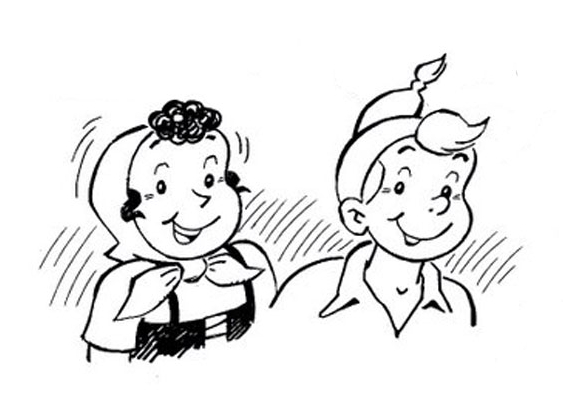
\includegraphics[width=.6\textwidth]{Sylvain+Sylvette_NB.jpg}} 
\newpage

\subsubsection{Exemple \no 7}

Sylvain part à bicyclette de A et se dirige vers B. Il roule à $20$ km/h.



Après avoir parcouru 8 km, il revient en A, s'arrête 12 minutes, puis repart vers B.

Sylvette va directement de A vers B. Elle roule à 16 km/h.

Sylvain et Sylvette sont partis en même temps de A et sont arrivés ensemble à B.

Quelle est la distance entre A et B ? 




\begin{enumerate}
\item \textbf{Choix de l'inconnue}

      Soit d la distance entre A et B. (l'unité est le kilomètre)

\item \textbf{ Mise en équation du problème}

Temps mis par Sylvain : $\dfrac{d+16}{20} + 0,2$

Temps mis par Sylvette : $\dfrac{d}{16}$

$\dfrac{d+16}{20} + \dfrac{1}{5} = \dfrac{d}{16} $


\item \textbf{ Résolution de l'équation}

$\dfrac{d+16}{20} + \dfrac{1}{5} = \dfrac{d}{16} $

$\dfrac{d+16}{20} + \dfrac{4}{20} = \dfrac{d}{16} $

$\dfrac{d+20}{20} = \dfrac{d}{16} $

$\dfrac{4\left(d+20\right)}{80} = \dfrac{5d}{80} $

$4\left(d+20\right) = 5d $

$ 4d + 80 = 5d$

$ -d = -80 $

$ d = 80 $

\item \textbf{ Réponse au problème}

La distance entre A et B est de 80 km.

\end{enumerate}


\newpage

\subsubsection{Exemple \no 8}



Sylvain et Sylvette partent simultanément pour effectuer un trajet de 54 km.


La vitesse de Sylvain est supérieure de 6 km/h à celle de Sylvette.

Sylvain arrive 45 min avant Sylvette.

Quelles sont les vitesses respectives de Sylvain et Sylvette ?



\begin{enumerate}
\item \textbf{Choix de l'inconnue}

Soit V la vitesse de Sylvette en km/h.

\item \textbf{Mise en équation du problème}

Temps mis par Sylvain : $\dfrac{54}{V+6}$

Temps mis par Sylvette : $\dfrac{54}{V}$

$\dfrac{54}{V+6} + \dfrac{3}{4} = \dfrac{54}{V}$

\item \textbf{Résolution de l'équation}

$\dfrac{54}{V+6} + \dfrac{3}{4} = \dfrac{54}{V}$

$\dfrac{216}{4V+24} + \dfrac{3V+18}{4V+24} = \dfrac{54}{V}$

$V\left(216+3V+18\right)=54\left(4V+24\right) $

$ 216V + 3V^2 + 18V = 216V + 1296 $

$ 3V^2 + 18V -1296 = 0 $

$ 3\left(V^2 + 6V - 432\right)=0 $

$ 3\left[\left(V^2 + 6V +9\right) - 441\right] = 0 $

$ 3\left(V+3\right)^2 - 21^2 = 0 $

$ 3\left(V + 3 + 21 \right)\left(V+3-21\right)=0 $

$ 3\left(V+24\right)\left(V-18\right) = 0 $ \\

\begin{tabular}{lcl}
$V+24 = 0$ & ou &$V-18=0$\\
$V=-24$ & ou &$V=18$\\
\end{tabular} \\

Une vitesse ne peut être négative, donc $V=18$.

On sait que la vitesse de Sylvain est $V+6$. Donc la vitesse de Sylvette est de 18 hm/h et celle de Sylvain 24 km/h.
\end{enumerate}



\ifdefined\COMPLETE
\else
    \end{document}
\fi